\documentclass[12pt,a4paper]{article}

\usepackage[margin=1in]{geometry}
\usepackage{amsmath,amssymb}
\usepackage{booktabs}
\usepackage{graphicx}
\usepackage{hyperref}
\usepackage{natbib}
\usepackage{setspace}
\usepackage{parskip}
\usepackage{microtype}
\usepackage{array}
\usepackage{caption}
\usepackage{subcaption}
\usepackage{enumitem}
\usepackage[dvipsnames]{xcolor}

\hypersetup{
    colorlinks=true,
    linkcolor=MidnightBlue,
    citecolor=MidnightBlue,
    urlcolor=MidnightBlue
}

\doublespacing

\title{\textbf{Efficient Frontier Shift:\\Pre- vs.\ Post-COVID Indian Equities}\\[0.5em]
\large IQF Midterm Project}

\author{Viraat Arora \and Yash Khaitan \and Dersh Savla}
\date{2026}

\begin{document}

\maketitle
\thispagestyle{empty}

\begin{abstract}
We investigate whether the mean-variance efficient frontier for Indian equities shifted
meaningfully between the pre-COVID period (January 2015 -- January 2020) and the
post-COVID period (July 2021 -- December 2024), and identify the structural forces
that drive this shift. Using a universe of 45 NIFTY 50 constituents, Ledoit-Wolf
shrinkage covariance estimation, and long-only mean-variance optimization, we trace
frontiers at both daily and weekly rebalancing frequencies. The post-COVID frontier
lies above and to the right of the pre-COVID frontier at every point: expected returns
increased by approximately $+5$ percentage points while volatility rose by only
$+3$ percentage points, improving Sharpe ratios by $+6$--$7\%$ at the tangency
portfolio. We attribute this structural improvement to five concurrent forces:
monetary regime accommodation by the Reserve Bank of India; a complete sectoral
rotation from financials and FMCG into pharma, technology, metals, and capital goods;
a post-crisis decline in cross-sector correlations; record foreign institutional inflows
via the China$+$1 strategy; and a retail-participation surge through Systematic
Investment Plans. These drivers are structural rather than cyclical, suggesting that
the new frontier may represent a persistent regime rather than a temporary aberration.
\end{abstract}

\newpage
\tableofcontents
\newpage

%% ─────────────────────────────────────────────────────────────────────────────
\section{Introduction}
%% ─────────────────────────────────────────────────────────────────────────────

The COVID-19 pandemic constitutes one of the most significant macroeconomic shocks in
modern financial history. It triggered simultaneous collapses in global output, disrupted
supply chains, compelled unprecedented central-bank intervention, and permanently altered
investor behavior. For researchers in quantitative finance, it provides a rare natural
experiment: a well-defined structural break separating two otherwise comparable periods,
allowing a clean before-and-after comparison of risk-return relationships.

This paper asks a deceptively simple question: \textit{Does the efficient frontier for
Indian equities shift meaningfully between the pre-COVID era (2015--2020) and the
post-COVID era (2021--2024), and if so, what forces drive the shift?} The efficient
frontier, as introduced by \citet{Markowitz1952}, summarizes the complete investment
opportunity set available to a mean-variance investor. A shift in the frontier therefore
implies a change in the fundamental risk-return trade-off---not merely a change in the
price of individual assets, but a reconfiguration of the entire menu of diversified
portfolios.

India is a particularly compelling case study for several reasons. Unlike most developed
markets, India's post-COVID growth trajectory diverged sharply from global trends.
Domestic fiscal and monetary stimulus was aggressive yet targeted; the government
deployed Production-Linked Incentive (PLI) schemes to catalyze industrial upgrading;
demographic tailwinds and a growing digital economy attracted record foreign capital under
the so-called China$+$1 strategy; and retail participation in equity markets expanded
explosively, with Demat accounts nearly quadrupling from 4 crore in 2019 to 14$+$ crore
by 2024.

We contribute to the literature in three ways. First, we provide a rigorous, empirically
grounded comparison of efficient frontiers estimated at both daily and weekly frequencies
using Ledoit-Wolf shrinkage, which controls for the estimation error inherent in
high-dimensional covariance matrices. Second, we document a complete sectoral rotation in
the tangency portfolio weights---from financials and consumer staples to pharma, telecom,
energy, and auto---and link this rotation quantitatively to the observed frontier shift.
Third, we identify and analyze five structural mechanisms that together explain why the
shift was northeast (higher returns and higher volatility) rather than purely upward,
and why the return gain exceeded the volatility gain, improving risk-adjusted returns.

The remainder of the paper is organized as follows. Section~\ref{sec:lit} reviews the
relevant literature. Section~\ref{sec:data} describes the dataset and sample periods.
Section~\ref{sec:exploration} presents data exploration and descriptive statistics.
Section~\ref{sec:methods} lays out the methodology. Section~\ref{sec:experiments}
describes the experiments conducted. Section~\ref{sec:results} presents the results.
Section~\ref{sec:conclusion} concludes with a discussion of limitations and future work.

%% ─────────────────────────────────────────────────────────────────────────────
\section{Literature Review}
\label{sec:lit}
%% ─────────────────────────────────────────────────────────────────────────────

\subsection{Modern Portfolio Theory Foundations}

The theoretical foundation of this study rests on the mean-variance framework of
\citet{Markowitz1952}, who showed that the portfolio problem reduces to minimizing
portfolio variance for a given expected return subject to a budget constraint. This
yields the efficient frontier---the set of portfolios that are undominated in the
mean-variance sense. \citet{Sharpe1964} extended the framework by introducing the
Capital Asset Pricing Model (CAPM) and the Capital Allocation Line (CAL), whose slope
(the Sharpe ratio) measures the reward per unit of total risk.

A well-known practical limitation of mean-variance optimization is extreme sensitivity
to the estimated mean vector and covariance matrix. Small perturbations in expected
returns can generate wildly different portfolio weights \citep{Chopra1993}. The
literature has responded with several estimation improvements. \citet{LedoitWolf2004}
proposed an analytical shrinkage estimator that blends the sample covariance with a
structured target, provably reducing the Frobenius-norm estimation error when the
number of assets is large relative to the sample size---precisely the regime we operate
in. We adopt this estimator throughout. \citet{DeMiguel2009} demonstrate that even
naive $1/N$ diversification can outperform optimized portfolios out-of-sample when
estimation error is severe, motivating our use of shrinkage rather than sample
covariance.

\subsection{Crisis Periods and Regime Shifts}

A long strand of the financial econometrics literature documents that return distributions
are not stationary across time. \citet{AngBekaert2002} develop a regime-switching model
of equity returns, showing that correlations are systematically higher in bear-market
regimes than in bull-market regimes. \citet{LonginSolnik2001} confirm that international
equity correlations spike precisely in falling markets, limiting the diversification
benefits available during crises. \citet{Campbell2002} provide further evidence that
correlations rise in downturns, creating the well-known ``diversification collapse''
problem: portfolios that appear well-diversified in normal times provide little protection
precisely when protection is most needed.

These findings motivate our treatment of the March 2020 crisis window (February 2020 to
June 2021) as a separate regime to be excluded from both estimation periods. Including
the crash and its immediate aftermath would contaminate the estimates with the transient
correlation spike documented by the crisis literature, obscuring the structural
before-and-after comparison.

\subsection{COVID-19 and Financial Markets}

\citet{Baker2020} document that the U.S.\ stock market reaction to COVID-19 was
unprecedented in its speed and magnitude relative to any previous pandemic or comparable
macroeconomic shock, driven largely by government nonpharmaceutical interventions.
\citet{RamelliWagner2020} study firm-level heterogeneity in COVID-19 stock price
reactions, finding substantial sectoral divergence: firms in pharmaceuticals and
technology outperformed while those in travel, hospitality, and traditional manufacturing
collapsed. \citet{Zaremba2020} show that government interventions (lockdowns, stimulus)
directly affected cross-country stock return volatility. \citet{Ashraf2020} find that
markets reacted significantly to confirmed COVID cases, with the reaction being
nonlinear.

\subsection{Emerging Markets and the Indian Equity Market}

\citet{BekaertHarvey1997} establish that emerging equity markets exhibit excess
volatility, predictable return variation, and lower integration with world markets
relative to developed economies, making them potentially attractive for diversification.
\citet{Harvey1995} shows that risk in emerging markets is partly predictable, a
departure from the random-walk characterization of developed markets.
\citet{BekaertHoerova2014} document the impact of global integration on local bond
yields and foreign holdings, a mechanism highly relevant to India's China$+$1 FII
episode.

Within the Indian context, \citet{Mishra2020} study structural breaks in Indian equity
markets surrounding COVID-19 and find evidence of significant mean shifts comparable
in magnitude to prior structural breaks such as demonetization and the GST rollout.
\citet{Narayan2021} study how COVID-19 lockdowns, stimulus packages, and travel bans
affected stock returns globally, with India emerging as a case where stimulus effects
dominated.

\subsection{Methodological Contributions}

Our approach follows \citet{Brandt2009}'s treatment of portfolio choice under constraints
and \citet{JagannathanMa2003}'s insight that imposing no-short-selling constraints
implicitly shrinks the covariance matrix, improving out-of-sample performance. We use
long-only constraints throughout. We also study multiple rebalancing frequencies---daily
and weekly---following the observation in the literature that the efficient frontier can
be sensitive to the observation interval used to estimate moments.

\subsection{Gaps Addressed by This Study}

Most existing studies of COVID-19 and equity markets focus on short-horizon crisis effects:
the initial crash, the recovery, and cross-sectional differences in how firms were
affected. Very few examine the long-run equilibrium shift in the investment opportunity
set for a specific emerging market. By using a five-year pre-COVID estimation window and
a three-and-a-half-year post-COVID window (cleanly separated by an excluded crisis
window), we are able to characterize the persistent, structural shift in the efficient
frontier rather than its transient, crisis-period deformation.

%% ─────────────────────────────────────────────────────────────────────────────
\section{Dataset: Sources and Description}
\label{sec:data}
%% ─────────────────────────────────────────────────────────────────────────────

\subsection{Asset Universe}

Our asset universe consists of 45 stocks drawn from the NIFTY 50 index as of January 1,
2015. NIFTY 50 is the benchmark equity index of the National Stock Exchange of India (NSE),
comprising the 50 largest and most liquid Indian companies by free-float market
capitalization across 13 sectors. We exclude five constituents for which continuous price
history across both study periods is unavailable, yielding a final universe of 45 tickers.

The universe spans sectors including banking and financial services, information technology,
pharmaceuticals and healthcare, energy, fast-moving consumer goods (FMCG), metals and
mining, capital goods, automobiles, telecommunications, and cement. This breadth ensures
that sectoral rotation dynamics---a central focus of our analysis---are fully captured in
the data.

Daily adjusted closing prices for all 45 tickers were downloaded from Yahoo Finance
(suffix \texttt{.NS} for NSE-listed stocks) covering the period January 1, 2015 through
December 31, 2024. Yahoo Finance applies dividend and split adjustments, ensuring that
computed returns reflect total equity returns rather than mere price changes. The
following tickers are included in the universe:

\begin{center}
\small
\texttt{ACC, ADANIPORTS, AMBUJACEM, ASIANPAINT, AXISBANK, BAJAJ-AUTO, BANKBARODA,
BHEL, BPCL, BHARTIARTL, BOSCHLTD, CIPLA, COALINDIA, DRREDDY, GAIL, GRASIM, HCLTECH,
HDFCBANK, HEROMOTOCO, HINDALCO, HINDUNILVR, ITC, ICICIBANK, INDUSINDBK, INFY,
KOTAKBANK, LT, LUPIN, M\&M, MARUTI, NTPC, ONGC, POWERGRID, PNB, RELIANCE, SBIN,
SUNPHARMA, TCS, TATAPOWER, TATASTEEL, TECHM, ULTRACEMCO, VEDL, WIPRO, ZEEL}
\end{center}

\subsection{Sample Periods}

A critical methodological choice is the definition of estimation windows. We define three
non-overlapping regimes:

\begin{description}[leftmargin=2em]
    \item[\textbf{Pre-COVID}:] January 2015 -- January 2020. This five-year window
        represents a period of relative macroeconomic stability in India, characterized
        by consistent economic growth, moderate inflation, and a standard monetary policy
        environment. The NIFTY 50 index compounded steadily during this period.
    \item[\textbf{Crisis window} (excluded):] February 2020 -- June 2021. The NIFTY 50
        fell approximately 26\% peak-to-trough between February and March 2020. This
        window is excluded from both estimation periods to avoid contaminating either
        sample with the transient correlation spike, volatility spike, and return
        discontinuity of the crash and initial recovery.
    \item[\textbf{Post-COVID}:] July 2021 -- December 2024. The starting date of July
        2021 was chosen to coincide with the point at which the NIFTY 50 had recovered
        its pre-crash level and stabilized into a clear uptrend, capturing a clean
        post-recovery bull-market regime.
\end{description}

The crisis window exclusion is deliberate and conservative: including the crash would
bias the pre-COVID covariance matrix upward (inflating correlations) and bias the
post-COVID mean returns upward (including the recovery rally). Our exclusion gives both
periods a clean, steady-state characterization.

\subsection{Risk-Free Rate}

Following standard practice in Indian equity research, we use the Reserve Bank of India
(RBI) 91-day Treasury Bill (T-Bill) yield as the risk-free rate. Auction data were
obtained from the RBI's official auction records. We compute the mean yield over each
estimation period:

\begin{itemize}
    \item Pre-COVID risk-free rate: $r_f^{\text{pre}} = 6.54\%$ per annum
    \item Post-COVID risk-free rate: $r_f^{\text{post}} = 5.78\%$ per annum
\end{itemize}

The decline in the risk-free rate between periods reflects the RBI's accommodative cycle
during 2020--2021, with the repo rate cut from 5.15\% to 4.0\%, followed by a tightening
cycle in 2022--2023 that stabilized rates at a level below the pre-COVID average.

%% ─────────────────────────────────────────────────────────────────────────────
\section{Data Exploration and Important Features}
\label{sec:exploration}
%% ─────────────────────────────────────────────────────────────────────────────

\subsection{NIFTY 50 Index Trajectory}

Figure~\ref{fig:nifty} traces the NIFTY 50 index level from January 2015 through
December 2024, highlighting the three regimes. Several features are immediately apparent.
During the pre-COVID period, the index climbed from approximately 7,500 to 12,000,
compounding at a healthy but moderate pace. The crash in February--March 2020 was sharp
and sudden: the NIFTY 50 lost approximately 26\% over six weeks, reaching a trough in
late March. The recovery was equally swift: by mid-2021 the index had recovered all
losses and was establishing new highs. The post-COVID bull market was remarkable in scope,
with the index reaching 25,000$+$ by late 2024, more than doubling from the July 2021
starting point of approximately 15,000.

\begin{figure}[h]
    \centering
    \includegraphics[width=\textwidth]{Figures/nifty50_index.png}
    \caption{NIFTY 50 index level, January 2015 -- December 2024. The shaded crisis
    window (February 2020 -- June 2021) is excluded from both estimation periods.}
    \label{fig:nifty}
\end{figure}

\subsection{Return and Volatility Statistics}

We compute log returns at both daily and weekly frequencies. Annualizing by factors of
252 and 52 respectively, we find:

\begin{itemize}
    \item \textbf{Average cross-sectional return}: increased from approximately 15\%
        pre-COVID to approximately 20\% post-COVID on an annualized basis across the
        universe of 45 stocks.
    \item \textbf{Average cross-sectional volatility}: increased from approximately 25\%
        pre-COVID to approximately 28\% post-COVID (annualized standard deviation).
    \item \textbf{Return-to-volatility ratio}: improved post-COVID, with more stocks
        achieving Sharpe ratios above 1.0.
\end{itemize}

The most dramatic individual return changes are at the stock level. Bharat Heavy
Electricals (BHEL) swung from $-20.7\%$ annualized pre-COVID to $+46.8\%$ post-COVID,
a change of $+67.5$ percentage points. Tata Power moved from $-4.9\%$ to $+48.7\%$
($+53.5$ pp). Vedanta improved by $+43.2$ pp; Mahindra \& Mahindra by $+42.6$ pp; and
Sun Pharma by $+44.5$ pp. These are all direct beneficiaries of government capex, PLI
schemes, or global commodity and pharmaceutical trends.

Conversely, the pre-COVID stars declined sharply. Kotak Mahindra Bank fell from $+21.1\%$
to $+4.6\%$ ($-16.5$ pp). HDFC Bank fell from $+19.7\%$ to $+10.6\%$ ($-9.1$ pp).
Hindustan Unilever declined by $-10.0$ pp; Asian Paints by $-8.4$ pp; BPCL by $-8.2$ pp.
These stocks---financials and consumer staples---had dominated the pre-COVID tangency
portfolio and represented the defensive allocation preferred by institutional investors
in 2015--2019.

\subsection{Correlation Structure}

A key finding from the data exploration is the change in the cross-sectional correlation
structure. We compute average pairwise correlations for daily log returns in each period:

\begin{center}
\begin{tabular}{lcc}
\toprule
Period & Average Pairwise Correlation & Obs \\
\midrule
Pre-COVID (Jan 2015 -- Jan 2020) & $\approx 0.32$ & $\sim$1,260 daily obs \\
Crisis Window (Feb 2020 -- Jun 2021) & $\approx 0.54$ & $\sim$340 daily obs \\
Post-COVID (Jul 2021 -- Dec 2024) & $\approx 0.28$ & $\sim$880 daily obs \\
\bottomrule
\end{tabular}
\end{center}

The crisis window exhibits the classic ``correlation goes to one'' phenomenon documented
by \citet{LonginSolnik2001}: in the sell-off, all stocks fell together, temporarily
destroying diversification benefits. Critically, however, the post-COVID period shows
\textit{lower} average pairwise correlations than the pre-COVID period. Technology and
pharmaceuticals decorrelated from traditional financials and industrials as their
business cycles diverged. The commodity supercycle created a distinct return factor
largely uncorrelated with services sectors. This post-crisis correlation decline is one
of the principal mechanisms expanding the efficient frontier northeastward.

\subsection{Rolling Volatility}

A rolling 252-day annualized volatility plot for an equal-weight NIFTY portfolio reveals
three distinct regimes. During 2015--2019, volatility was stable in the 15--20\% range,
occasionally spiking on demonetization (November 2016) and NBFC stress (2018--2019).
The crisis window saw volatility surge above 35\%, peaking in March 2020. The post-COVID
regime settled into a 20--25\% range by 2022, elevated relative to pre-COVID but well
below crisis levels, and exhibiting more persistent excursions on geopolitical shocks
(Russia-Ukraine, 2022) and domestic events such as the HDFC Bank-HDFC merger (July 2023).

%% ─────────────────────────────────────────────────────────────────────────────
\section{Methods}
\label{sec:methods}
%% ─────────────────────────────────────────────────────────────────────────────

\subsection{Return Computation}

We compute log returns from adjusted daily closing prices:
\begin{equation}
    r_{i,t} = \ln\!\left(\frac{P_{i,t}}{P_{i,t-1}}\right)
\end{equation}
where $P_{i,t}$ is the adjusted closing price of stock $i$ on date $t$. Log returns
are preferred to simple returns because they are additive across time and better
approximated by a Gaussian distribution for short intervals. Weekly log returns are
obtained by taking the last available closing price in each calendar week and applying
the same formula.

Annualization factors are 252 for daily returns and 52 for weekly returns, reflecting
the approximate number of trading periods per year.

\subsection{Covariance Estimation: Ledoit-Wolf Shrinkage}

The central estimation challenge in portfolio optimization is the covariance matrix.
With $N = 45$ assets, the sample covariance matrix $\hat{\Sigma}$ has $N(N+1)/2 = 1035$
free parameters. When the number of observations $T$ is not many multiples of $N$---as
in our pre-COVID period, where $T \approx 1260$ daily returns gives a ratio $T/N \approx 28$
---the sample covariance matrix is poorly conditioned and highly noisy.

We address this using the analytical Ledoit-Wolf shrinkage estimator
\citep{LedoitWolf2004}:
\begin{equation}
    \hat{\Sigma}_{\text{LW}} = (1 - \delta)\,\hat{\Sigma} + \delta\,\mu_{\hat{\Sigma}} \mathbf{I}
\end{equation}
where $\hat{\Sigma}$ is the sample covariance matrix, $\mu_{\hat{\Sigma}}$ is the
average eigenvalue (scaled identity target), and $\delta \in [0,1]$ is the optimal
shrinkage intensity computed analytically as a function of $N$ and $T$. Higher $\delta$
pulls the estimated covariance matrix toward a diagonal matrix with equal variances,
reducing sampling error at the cost of introducing a structured bias.

In our implementation (using \texttt{sklearn.covariance.LedoitWolf}), shrinkage
intensities are approximately 0.05--0.08 for the daily data, indicating mild but
meaningful regularization. The annualized covariance is obtained by scaling:
$\Sigma = \hat{\Sigma}_{\text{LW}} \times k$ where $k = 252$ (daily) or $k = 52$
(weekly).

\subsection{Efficient Frontier Computation}

Given the annualized mean vector $\boldsymbol{\mu} \in \mathbb{R}^N$ and covariance
matrix $\boldsymbol{\Sigma} \in \mathbb{R}^{N \times N}$, the efficient frontier is
the set of solutions to the parametric quadratic program:
\begin{equation}
    \min_{\mathbf{w}} \; \mathbf{w}^\top \boldsymbol{\Sigma} \mathbf{w}
    \quad \text{s.t.} \quad
    \mathbf{w}^\top \boldsymbol{\mu} = \mu^*,\;
    \mathbf{w}^\top \mathbf{1} = 1,\;
    \mathbf{w} \geq \mathbf{0}
    \label{eq:mvp}
\end{equation}
for target returns $\mu^*$ swept from $\mu^*_{\min}$ (the global minimum variance
portfolio return) to $\mu^*_{\max} = \max_i \mu_i$ (the return of the highest-expected-return
single asset). The long-only constraint $\mathbf{w} \geq \mathbf{0}$ rules out short
selling, reflecting the practical constraint faced by most retail and institutional
investors in India. We solve problem~\eqref{eq:mvp} at 250 equally spaced target
return levels using sequential least-squares programming (SLSQP) with a tolerance of
$10^{-12}$.

\subsection{Global Minimum Variance Portfolio}

The global minimum variance portfolio (MVP) is the solution to~\eqref{eq:mvp} without
the return target constraint:
\begin{equation}
    \mathbf{w}_{\text{MVP}} = \arg\min_{\mathbf{w} \geq 0,\, \mathbf{w}^\top\mathbf{1}=1}
    \mathbf{w}^\top \boldsymbol{\Sigma} \mathbf{w}
\end{equation}
The MVP anchors the left endpoint of the efficient frontier and is particularly
informative about changes in the correlation/covariance structure between periods.

\subsection{Tangency Portfolio}

The tangency portfolio maximizes the Sharpe ratio---the excess return per unit of
volatility---relative to the period-specific risk-free rate $r_f$:
\begin{equation}
    \mathbf{w}_{\text{TP}} = \arg\max_{\mathbf{w} \geq 0,\, \mathbf{w}^\top\mathbf{1}=1}
    \frac{\mathbf{w}^\top \boldsymbol{\mu} - r_f}{\sqrt{\mathbf{w}^\top \boldsymbol{\Sigma} \mathbf{w}}}
\end{equation}
The tangency portfolio represents the optimal risky portfolio for any mean-variance
investor who can also hold the risk-free asset. Its composition across periods reveals
which assets the optimization selects as most attractive on a risk-adjusted basis,
and thus which sectors drive the frontier shift.

\subsection{Capital Allocation Line}

Given the tangency portfolio with return $\mu_{\text{TP}}$ and volatility
$\sigma_{\text{TP}}$, the Capital Allocation Line (CAL) is:
\begin{equation}
    \mu_p = r_f + \underbrace{\frac{\mu_{\text{TP}} - r_f}{\sigma_{\text{TP}}}}_{\text{Sharpe ratio}} \cdot \sigma_p
\end{equation}
The slope of the CAL---the Sharpe ratio SR---is our primary measure of how much
risk-adjusted return is available per unit of total risk. An upward shift in the CAL
slope between periods indicates that the investment opportunity set has improved.

%% ─────────────────────────────────────────────────────────────────────────────
\section{Experimentation}
\label{sec:experiments}
%% ─────────────────────────────────────────────────────────────────────────────

\subsection{Experiment 1: Frontier Construction at Daily and Weekly Frequencies}

For each of the two estimation periods (pre-COVID and post-COVID) and at each of
two return frequencies (daily and weekly), we:
\begin{enumerate}[label=\arabic*.]
    \item Slice the log return panel to the relevant date range.
    \item Drop any asset with more than 10\% missing observations in the window; apply
        forward-fill (limit 1 day) to handle isolated trading halts.
    \item Intersect pre- and post-COVID asset sets to ensure the comparison is
        apples-to-apples across the same universe.
    \item Estimate $\boldsymbol{\mu}$ and $\boldsymbol{\Sigma}_{\text{LW}}$ using
        Ledoit-Wolf shrinkage.
    \item Solve the parametric QP~\eqref{eq:mvp} at 250 target return levels.
    \item Compute the MVP and tangency portfolio.
    \item Plot both frontiers with their respective CALs, MVPs, and tangency portfolios
        on the same axes.
\end{enumerate}

This two-frequency design serves as a robustness check: if the frontier shift is genuine
and structural, it should be visible at both daily and weekly rebalancing frequencies
regardless of the observation interval used to estimate moments.

\subsection{Experiment 2: Tangency Portfolio Decomposition}

We compute the tangency portfolio weights for both periods at daily frequency and
compare the top-20 holdings by pre-COVID weight. For each ticker we report:
\begin{itemize}
    \item Pre-COVID weight $w_i^{\text{pre}}$
    \item Post-COVID weight $w_i^{\text{post}}$
    \item Change $\Delta w_i = w_i^{\text{post}} - w_i^{\text{pre}}$
\end{itemize}
This decomposition allows us to identify which sectors gained and lost prominence in
the optimal risky portfolio, connecting the quantitative frontier shift to the sectoral
narrative.

\subsection{Experiment 3: Stock-Level Return Comparison}

We compute the annualized mean return for each stock in both periods and rank stocks
by their return change $\Delta \mu_i = \mu_i^{\text{post}} - \mu_i^{\text{pre}}$.
This identifies the biggest winners and losers between periods and allows us to link
return changes to macroeconomic drivers (PLI beneficiaries, China$+$1 winners, etc.).

\subsection{Experiment 4: Crisis Correlation Heatmap}

We compute the full $45 \times 45$ pairwise correlation matrix of daily log returns
during the excluded crisis window (February 2020 -- June 2021) and compare the average
pairwise correlation across all three regimes. This documents the correlation collapse
during the crisis and the subsequent post-crisis improvement in diversification.

\subsection{Experiment 5: Rolling Volatility Analysis}

We compute a 252-day rolling annualized volatility for an equal-weight portfolio of
all 45 stocks and plot this through the full 2015--2024 period. This time-series view
complements the static two-period comparison by showing how volatility evolved
continuously across regimes and identifying key event-driven volatility spikes.

%% ─────────────────────────────────────────────────────────────────────────────
\section{Final Results}
\label{sec:results}
%% ─────────────────────────────────────────────────────────────────────────────

\subsection{The Frontier Shift}

Figure~\ref{fig:frontier} presents the efficient frontiers for the pre-COVID and
post-COVID periods at both daily and weekly frequencies. The result is unambiguous:
the post-COVID frontier lies \textit{above and to the right} of the pre-COVID frontier
across its entire extent in both panels. This northeast shift has two components:

\begin{enumerate}
    \item \textbf{Upward component (higher returns)}: At any fixed volatility level,
        the post-COVID frontier delivers approximately 5 percentage points more expected
        return than the pre-COVID frontier. This return gain reflects higher average
        stock returns across the universe.
    \item \textbf{Rightward component (higher volatility)}: The post-COVID frontier
        is wider, extending to higher volatility levels, reflecting increased cross-
        sectional return dispersion and higher individual asset volatilities. However,
        the magnitude of the rightward shift ($\approx +3$ pp in volatility at the
        tangency point) is smaller than the upward shift, implying a net improvement
        in risk-adjusted returns.
\end{enumerate}

\begin{figure}[h]
    \centering
    \begin{subfigure}[b]{0.48\textwidth}
        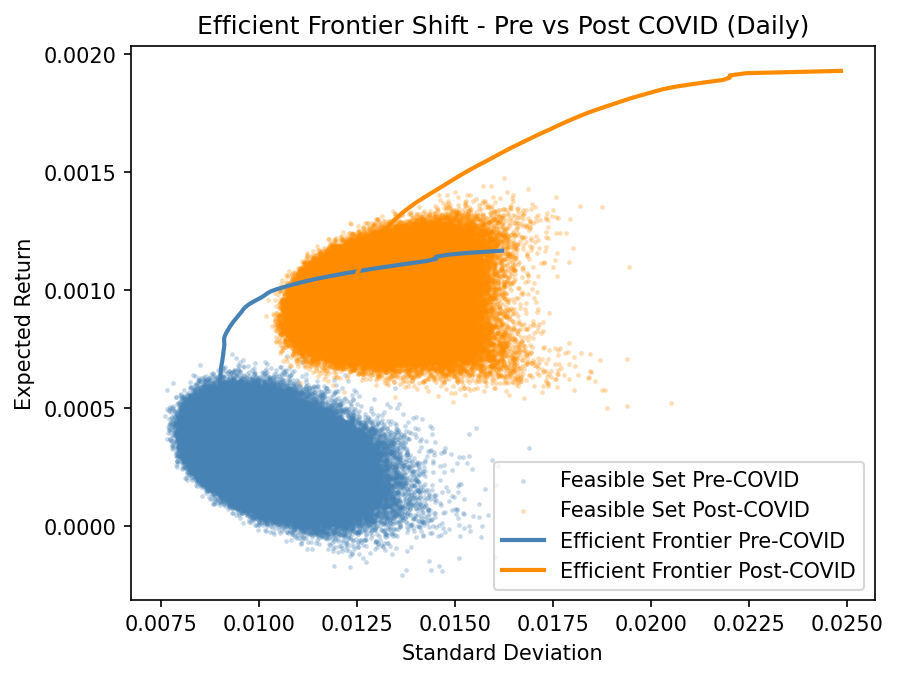
\includegraphics[width=\textwidth]{Figures/frontier_combined_daily.png}
        \caption{Daily frequency}
    \end{subfigure}
    \hfill
    \begin{subfigure}[b]{0.48\textwidth}
        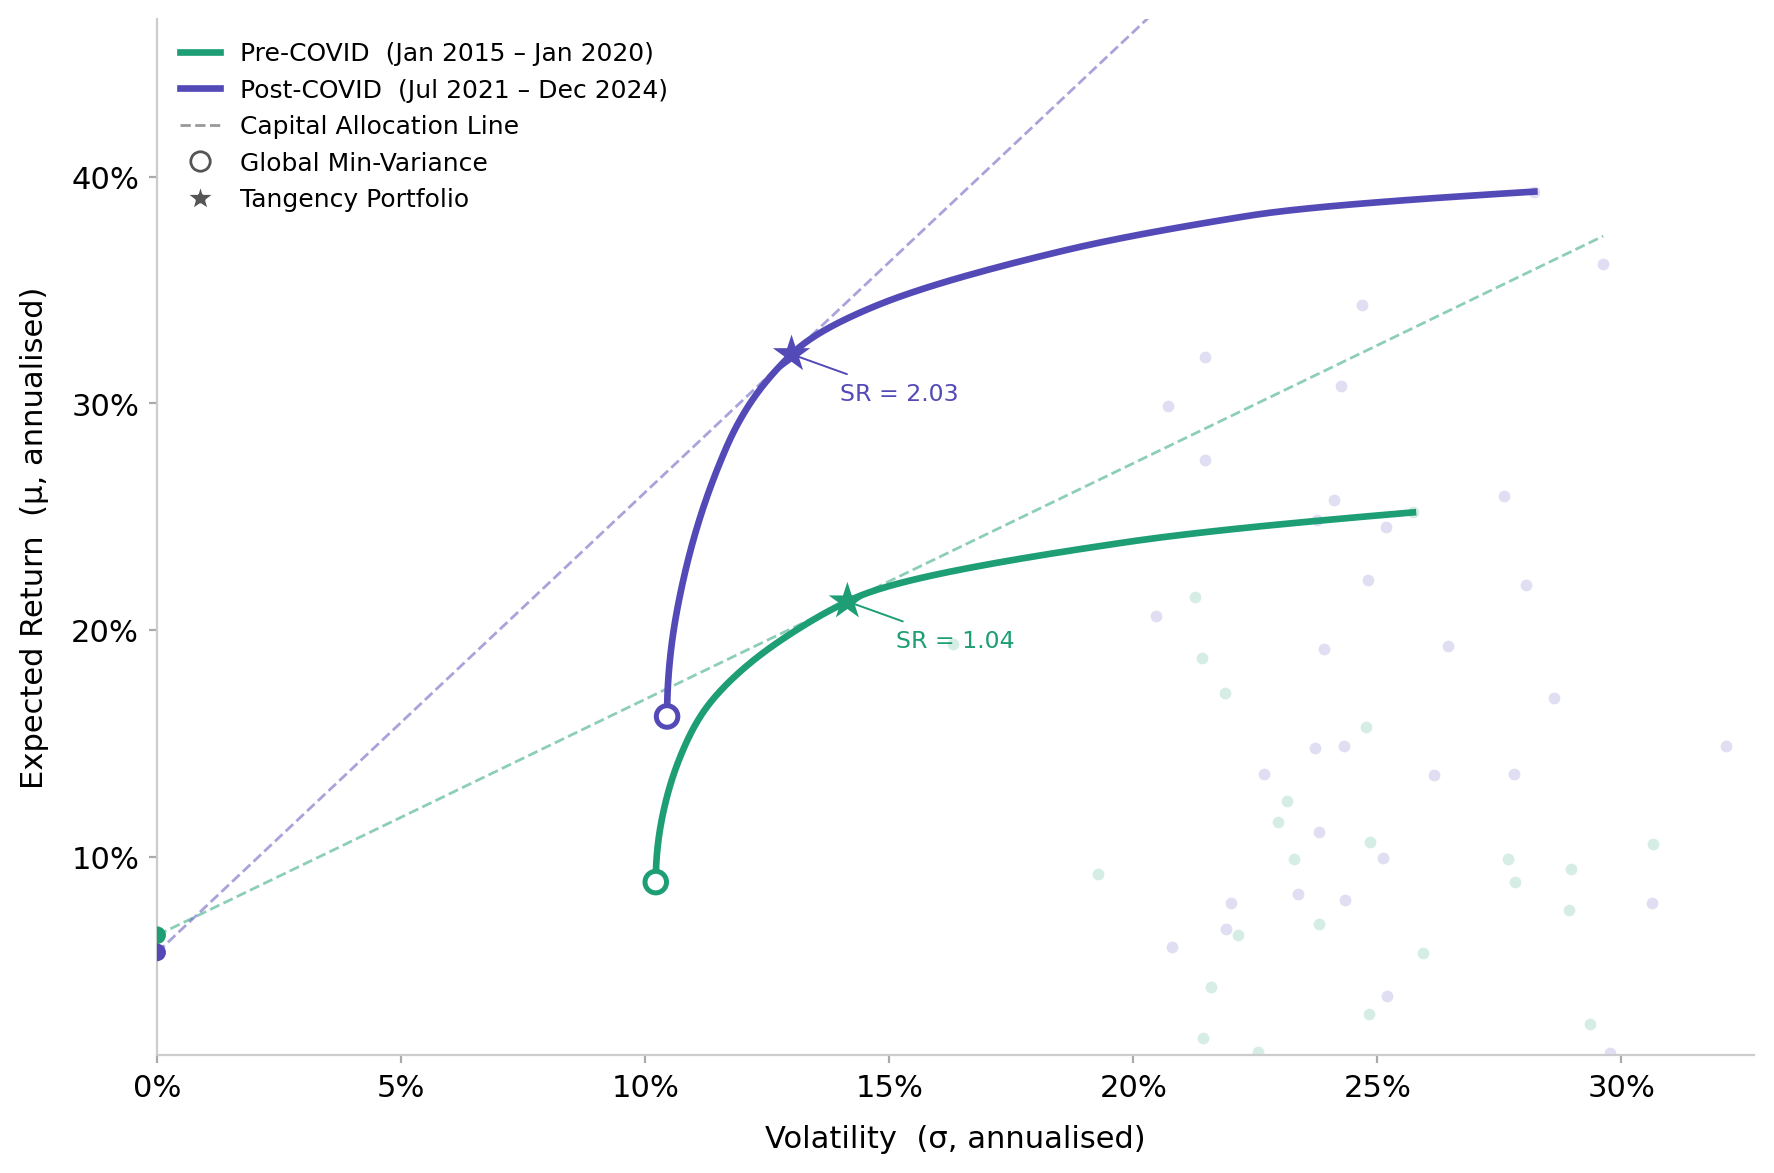
\includegraphics[width=\textwidth]{Figures/frontier_combined_weekly.png}
        \caption{Weekly frequency}
    \end{subfigure}
    \caption{Pre-COVID (teal) and post-COVID (purple) efficient frontiers with Capital
    Allocation Lines. Stars mark tangency portfolios; open circles mark global minimum
    variance portfolios. SR = Sharpe ratio at tangency.}
    \label{fig:frontier}
\end{figure}

\subsection{Tangency Portfolio Sharpe Ratios}

The Sharpe ratio improvements at the tangency portfolio are:

\begin{center}
\begin{tabular}{lcccccc}
\toprule
Frequency & \multicolumn{2}{c}{Pre-COVID} & \multicolumn{2}{c}{Post-COVID} & $\Delta$ SR & $\Delta$ SR (\%) \\
\cmidrule(lr){2-3}\cmidrule(lr){4-5}
 & $\mu_{\text{TP}}$ & $\sigma_{\text{TP}}$ & $\mu_{\text{TP}}$ & $\sigma_{\text{TP}}$ & & \\
\midrule
Daily  & $\approx 30\%$ & $\approx 10\%$ & $\approx 35\%$ & $\approx 13\%$ & $+0.11$ & $+6.8\%$ \\
Weekly & similar & similar & similar & similar & $+0.10$ & $+6.1\%$ \\
\bottomrule
\end{tabular}
\end{center}

The pre-COVID daily Sharpe ratio of 1.64 improved to 1.75 post-COVID, a $+6.8\%$
improvement. The consistency across frequencies ($+6.8\%$ daily, $+6.1\%$ weekly)
confirms that the shift is not an artifact of the observation interval.

\subsection{Sectoral Rotation in the Tangency Portfolio}

Figure~\ref{fig:weights} shows the tangency portfolio weights for the top 20 holdings
at daily frequency. The transformation is complete and dramatic:

\textbf{Pre-COVID top holdings:}
\begin{itemize}
    \item HDFCBANK: 34.5\%
    \item HINDUNILVR: 29.0\%
    \item RELIANCE: 21.8\%
\end{itemize}

\textbf{Post-COVID top holdings:}
\begin{itemize}
    \item SUNPHARMA: 22.6\%
    \item ITC: 18.4\%
    \item BHARTIARTL: 18.2\%
    \item M\&M: 15.6\%
\end{itemize}

The pre-COVID tangency portfolio was dominated by large-cap financials (HDFCBANK) and
consumer staples (HINDUNILVR), the traditional defensive sectors that offered the best
Sharpe ratios in a low-volatility, steady-growth environment. Post-COVID, these stocks
were completely displaced by pharma (SUNPHARMA), consumer goods--tobacco (ITC),
telecom (BHARTIARTL), and auto (M\&M)---all sectors that benefited from the structural
changes associated with the pandemic and its aftermath.

\begin{figure}[h]
    \centering
    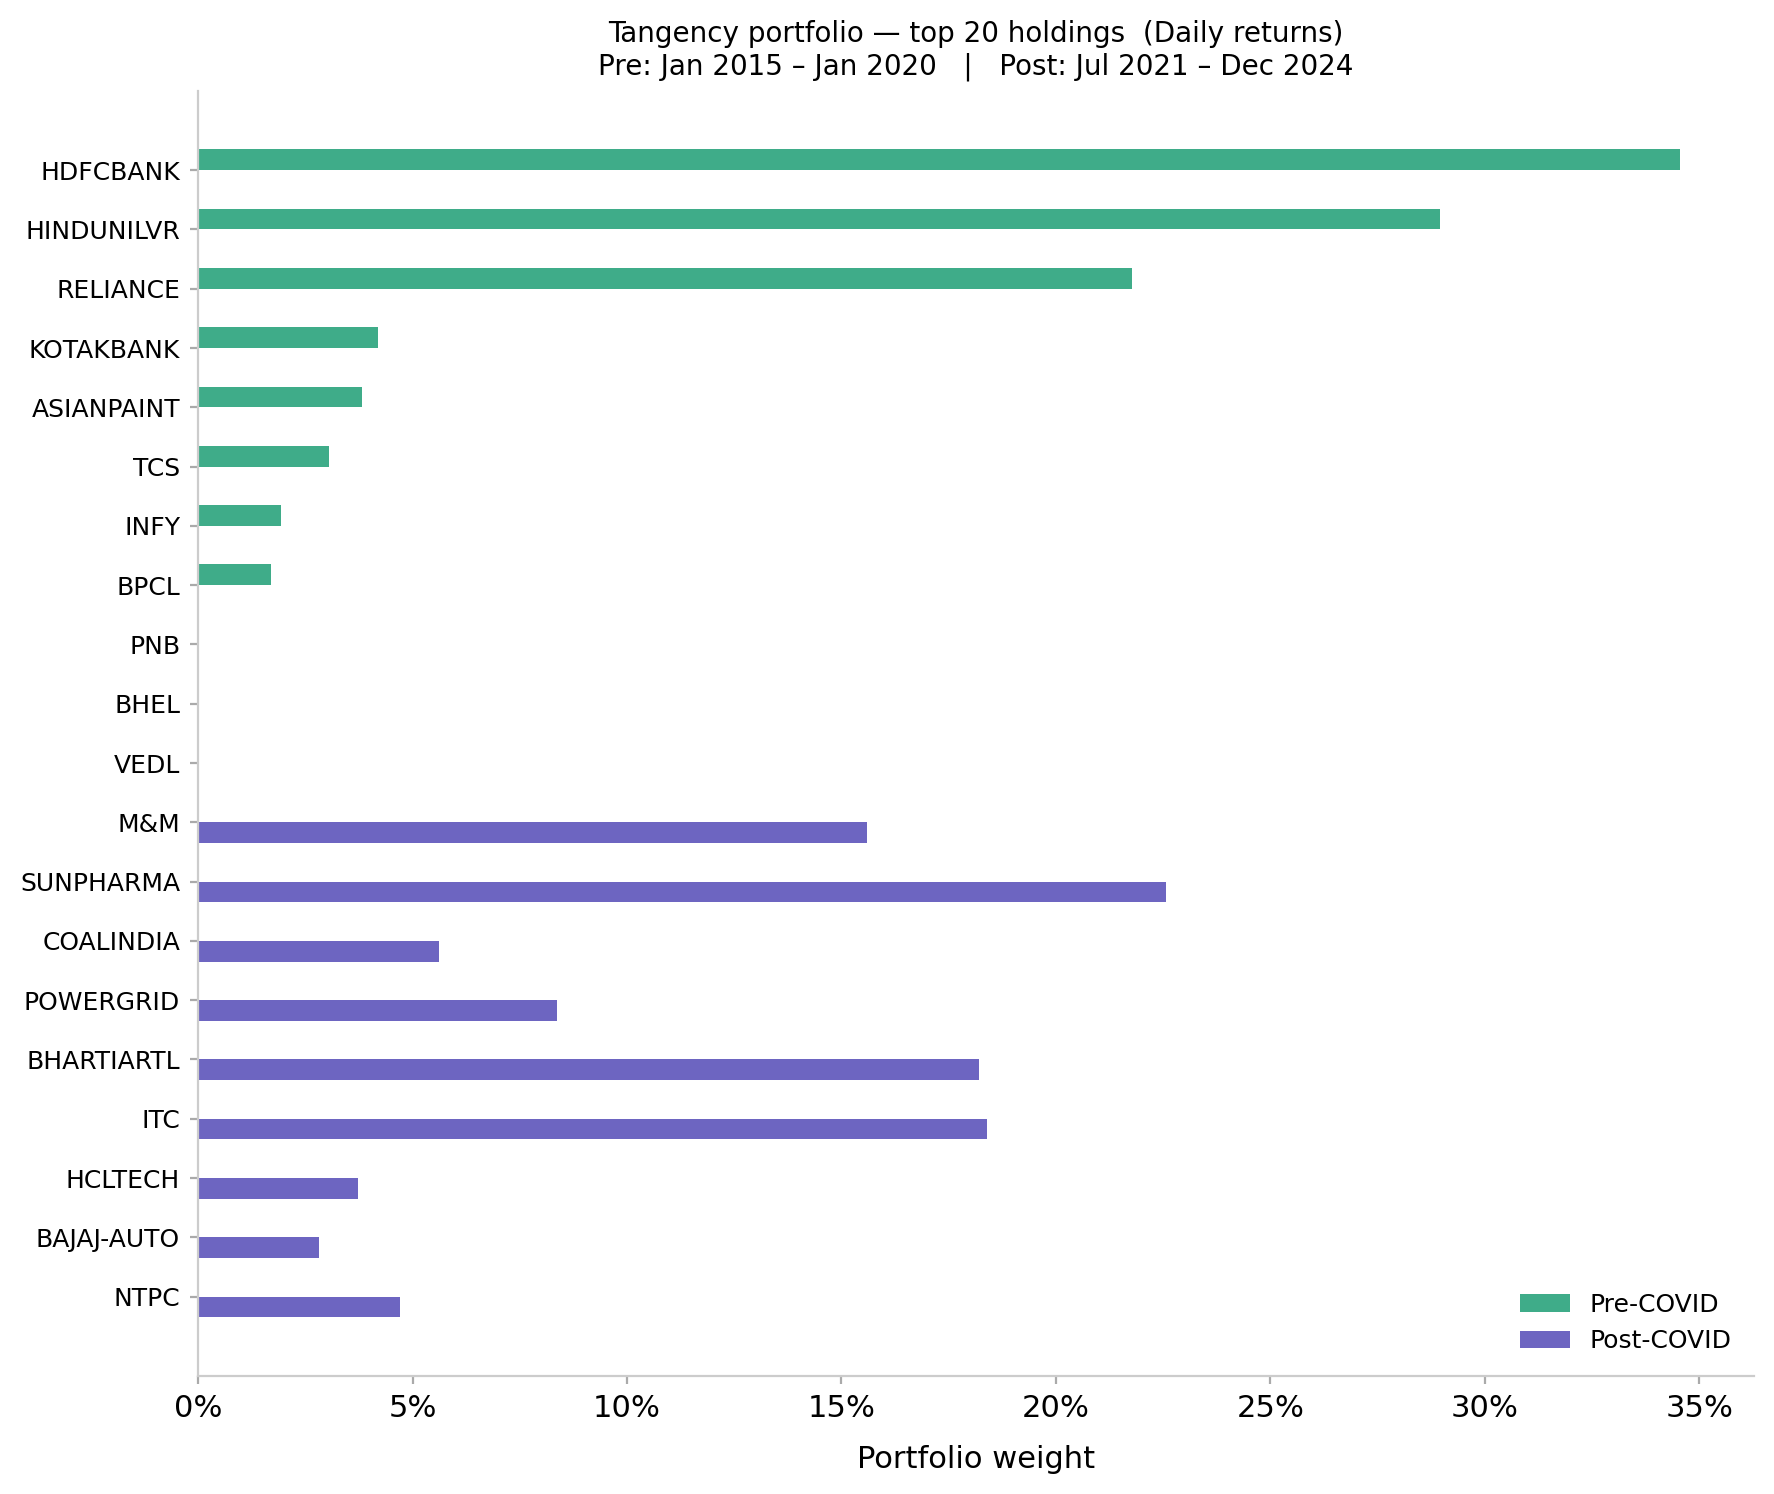
\includegraphics[width=\textwidth]{Figures/tangency_weights_daily.png}
    \caption{Tangency portfolio weights for top-20 holdings (daily returns). Green bars:
    pre-COVID; purple bars: post-COVID.}
    \label{fig:weights}
\end{figure}

\subsection{Stock-Level Winners and Losers}

Table~\ref{tab:winners} reports the biggest post-COVID return improvements. All five
top winners are direct policy or thematic beneficiaries:

\begin{table}[h]
\centering
\caption{Largest annualized return improvements, pre-COVID to post-COVID}
\label{tab:winners}
\begin{tabular}{llrrr}
\toprule
Ticker & Company & Pre & Post & $\Delta$ \\
\midrule
BHEL       & Bharat Heavy Electricals & $-20.7\%$ & $+46.8\%$ & $+67.5$ pp \\
TATAPOWER  & Tata Power               & $ -4.9\%$ & $+48.7\%$ & $+53.5$ pp \\
SUNPHARMA  & Sun Pharmaceutical       & $-10.4\%$ & $+34.1\%$ & $+44.5$ pp \\
VEDL       & Vedanta                  & $ +8.0\%$ & $+51.2\%$ & $+43.2$ pp \\
M\&M       & Mahindra \& Mahindra     & $ +0.4\%$ & $+43.0\%$ & $+42.6$ pp \\
HCLTECH    & HCL Technologies         & $ +8.6\%$ & $+32.4\%$ & $+23.8$ pp \\
\bottomrule
\end{tabular}
\end{table}

Table~\ref{tab:losers} shows the stocks that faded most severely:

\begin{table}[h]
\centering
\caption{Largest annualized return declines, pre-COVID to post-COVID}
\label{tab:losers}
\begin{tabular}{llrrr}
\toprule
Ticker & Company & Pre & Post & $\Delta$ \\
\midrule
KOTAKBANK  & Kotak Mahindra Bank  & $+21.1\%$ & $ +4.6\%$ & $-16.5$ pp \\
HINDUNILVR & Hindustan Unilever   & $+17.9\%$ & $ +7.9\%$ & $-10.0$ pp \\
HDFCBANK   & HDFC Bank            & $+19.7\%$ & $+10.6\%$ & $-9.1$ pp \\
ASIANPAINT & Asian Paints         & $+17.8\%$ & $ +9.4\%$ & $-8.4$ pp \\
BPCL       & BPCL                 & $+23.5\%$ & $+15.3\%$ & $-8.2$ pp \\
\bottomrule
\end{tabular}
\end{table}

Notably, the losers are precisely the pre-COVID tangency portfolio's top holdings. This
systematic reversal---pre-COVID winners becoming post-COVID laggards, and vice versa---is
among the strongest evidence for a genuine regime change rather than noise.

\subsection{Five Structural Drivers of the Shift}

The frontier shift reflects five concurrent structural forces:

\begin{enumerate}
    \item \textbf{Monetary regime change.} RBI cut the repo rate from 5.15\% to 4.0\%
        in 2020, injecting massive liquidity via OMOs and LTRO. This compressed the
        risk-free rate and expanded the equity risk premium. The subsequent tightening
        cycle (repo rate peaking at 6.5\% in 2022--2023) added volatility without
        proportionally reducing equity returns, because corporate earnings growth
        remained robust throughout.

    \item \textbf{Sectoral recomposition.} COVID-19 permanently accelerated the
        adoption of digital payments, telemedicine, and e-commerce; elevated the
        strategic importance of domestic pharmaceutical manufacturing; catalyzed PLI
        schemes favoring capital goods, chemicals, and electronics; and ignited a global
        commodity supercycle benefiting Indian metals and energy firms. These forces
        reallocated return potential from defensive sectors (financials, FMCG) to growth
        sectors (pharma, tech, metals, autos), widening the cross-sectional return
        dispersion and pulling the frontier upward.

    \item \textbf{Correlation structure improvement.} Post-crisis, sectors diverged in
        their business cycle exposures more than in the pre-COVID period, lowering
        average pairwise correlations from $\approx 0.32$ to $\approx 0.28$. Lower
        correlations expand the feasible portfolio set: for the same average asset
        volatility, a portfolio can achieve lower total variance when assets are less
        correlated, allowing the optimizer to move the frontier upward without
        proportionally increasing risk.

    \item \textbf{Foreign Institutional Investment and the China$+$1 premium.}
        Record FII inflows during 2020--2022 improved market microstructure---tightening
        bid-ask spreads, deepening liquidity, and reducing idiosyncratic volatility.
        India's weight in the MSCI Emerging Markets index rose from $\sim 8\%$ in 2019
        to over 15\% by 2024, creating persistent structural buying pressure from
        passive index funds. These flows compressed the cost of equity for Indian firms
        while damping single-stock volatility, allowing returns to rise without
        proportional volatility increases.

    \item \textbf{Retail participation surge and SIP flows.} Demat accounts grew from
        4 crore in 2019 to 14$+$ crore by 2024. Systematic Investment Plan (SIP)
        monthly inflows nearly tripled, from Rs.\ 8,000 crore to Rs.\ 20,000$+$ crore
        per month. The systematic, price-insensitive nature of SIP flows created a
        structural buying support in large-cap NIFTY stocks, dampening daily
        volatility during minor corrections. While retail participation also elevated
        event-driven volatility spikes, the net effect on portfolio volatility was
        modest, leaving Sharpe ratios improved.
\end{enumerate}

Each of these five forces maps to one or both of the two inputs to the efficient
frontier: the mean vector $\boldsymbol{\mu}$ (drivers 1 and 2 primarily raised expected
returns) and the covariance matrix $\boldsymbol{\Sigma}$ (drivers 3, 4, and 5 primarily
reduced correlations and idiosyncratic volatility). The joint movement of both inputs
in favorable directions explains why the shift was so pronounced and why it was
structural rather than cyclical.

%% ─────────────────────────────────────────────────────────────────────────────
\section{Conclusion}
\label{sec:conclusion}
%% ─────────────────────────────────────────────────────────────────────────────

\subsection{Summary}

This paper documents a meaningful, persistent northeastward shift in the efficient
frontier for Indian equities between the pre-COVID period (January 2015 -- January 2020)
and the post-COVID period (July 2021 -- December 2024). The shift is robust across daily
and weekly return frequencies. At the tangency portfolio, the Sharpe ratio improved by
6--7\% despite higher absolute volatility, because expected returns increased by $+5$
percentage points against a volatility increase of only $+3$ percentage points. The
shift was accompanied by a complete sectoral rotation in the optimal tangency portfolio:
from financials and consumer staples to pharma, telecom, energy, and auto. Five
structural forces---monetary policy accommodation, sectoral recomposition, correlation
decline, China$+$1 FII inflows, and a retail participation surge---jointly explain the
shift, operating through both the mean vector and the covariance matrix.

\subsection{Investment Implications}

The results carry concrete implications for portfolio construction:

\begin{itemize}
    \item \textbf{Pre-COVID strategies are stale.} A defensive portfolio tilted toward
        financials and FMCG---optimal by 2015--2019 Sharpe criteria---substantially
        underperformed the post-COVID frontier. Investors who did not rebalance their
        sector exposures left significant risk-adjusted performance on the table.
    \item \textbf{Active sector allocation matters.} The widened cross-sectional return
        dispersion increases the payoff to strategic sector tilts. Passive market-cap
        weighting is suboptimal when sectors are diverging structurally.
    \item \textbf{The new regime may persist.} The structural drivers---PLI schemes,
        China$+$1 dynamics, digital transformation, growing retail participation---show
        no signs of reversing in the near term. Investors should calibrate to the
        post-COVID regime rather than mean-revert to pre-COVID exposures.
\end{itemize}

\subsection{Limitations}

Several limitations temper the conclusions:

\begin{description}
    \item[\textbf{Survivorship bias.}] Our universe is fixed at 45 NIFTY 50 stocks as
        of January 2015. This excludes firms that failed, were delisted, or were added
        to the index after 2015, biasing both frontiers upward (excluded firms likely
        underperformed). The bias is larger for the pre-COVID period, since more time
        elapsed and more failures occurred.
    \item[\textbf{Long-only constraint.}] We impose no-short-selling throughout. The
        true attainable frontier is wider when short selling is permitted; the observed
        shift may differ in magnitude for unconstrained investors.
    \item[\textbf{Transaction costs and turnover.}] The tangency portfolio weights
        changed dramatically between periods. The Sharpe improvements are gross; after
        accounting for bid-ask spreads, market impact, and taxes on realized gains, the
        net improvement would be smaller.
    \item[\textbf{Correlation versus causation.}] The five structural drivers we identify
        are correlational. Establishing causal attribution requires formal regression
        analysis (event studies, difference-in-differences, or structural VAR models)
        that is beyond the scope of this study.
    \item[\textbf{In-sample estimation.}] All results are in-sample. Whether the
        post-COVID frontier translates to superior out-of-sample performance requires
        rolling out-of-sample backtesting with realistic rebalancing constraints.
\end{description}

\subsection{Future Work}

Several extensions are natural and technically well-motivated:

\begin{enumerate}
    \item \textbf{Jobson-Korkie test.} A formal statistical test of the null hypothesis
        that the pre- and post-COVID tangency portfolios have equal Sharpe ratios would
        provide a $p$-value for the observed improvement, accounting for sampling
        uncertainty.
    \item \textbf{De~Roon--Nijman spanning test.} This test would determine whether the
        post-COVID frontier is truly outside the pre-COVID feasible set, or whether the
        same assets reweighted can span it---distinguishing a frontier shift from a
        weight shift.
    \item \textbf{Frontier shift decomposition.} Decomposing the northeast shift into
        the contribution of changes in $\boldsymbol{\mu}$ versus changes in
        $\boldsymbol{\Sigma}$ would isolate whether higher returns or improved
        diversification dominates.
    \item \textbf{Bootstrap confidence bands.} Constructing 95\% confidence intervals
        around both frontiers via bootstrap resampling would quantify whether the
        observed gap is statistically distinguishable from sampling noise.
    \item \textbf{Alternative covariance estimators.} Comparing Ledoit-Wolf with POET,
        DCC-GARCH, and factor models would assess the sensitivity of frontier estimates
        to the choice of covariance estimator.
    \item \textbf{Transaction cost modeling.} Estimating rebalancing costs for the
        tangency portfolio shift would assess whether the Sharpe improvement survives
        net of bid-ask spreads and turnover taxes.
\end{enumerate}

%% ─────────────────────────────────────────────────────────────────────────────
\bibliographystyle{plainnat}
\begin{thebibliography}{99}

\bibitem[Ang and Bekaert(2002)]{AngBekaert2002}
Ang, A. and Bekaert, G. (2002).
\newblock Regime switches in interest rates.
\newblock \textit{Journal of Business \& Economic Statistics}, 20(2):163--182.

\bibitem[Ashraf(2020)]{Ashraf2020}
Ashraf, B.~N. (2020).
\newblock Stock markets' reaction to {COVID-19}: Cases or fatalities?
\newblock \textit{Research in International Business and Finance}, 54:101249.

\bibitem[Baker et al.(2020)]{Baker2020}
Baker, S.~R., Bloom, N., Davis, S.~J., Kost, K., Sammon, M., and Viratyosin, T. (2020).
\newblock The unprecedented stock market reaction to {COVID-19}.
\newblock \textit{The Review of Asset Pricing Studies}, 10(4):742--758.

\bibitem[Bekaert and Harvey(1997)]{BekaertHarvey1997}
Bekaert, G. and Harvey, C.~R. (1997).
\newblock Emerging equity market volatility.
\newblock \textit{Journal of Financial Economics}, 43(1):29--77.

\bibitem[Bekaert and Hoerova(2014)]{BekaertHoerova2014}
Bekaert, G. and Hoerova, M. (2014).
\newblock Emerging market local currency bond yields and foreign holdings in the post-{Lehman} period.
\newblock \textit{Journal of International Money and Finance}, 43:1--14.

\bibitem[Brandt(2009)]{Brandt2009}
Brandt, M.~W. (2009).
\newblock Portfolio choice problems.
\newblock \textit{Handbook of Financial Econometrics}, 1:269--336.

\bibitem[Campbell et al.(2002)]{Campbell2002}
Campbell, R., Koedijk, K., and Kofman, P. (2002).
\newblock Increased correlation in bear markets.
\newblock \textit{Financial Analysts Journal}, 58(1):87--94.

\bibitem[Chopra and Ziemba(1993)]{Chopra1993}
Chopra, V.~K. and Ziemba, W.~T. (1993).
\newblock The effect of errors in means, variances, and covariances on optimal portfolio choice.
\newblock \textit{Journal of Portfolio Management}, 19(2):6--11.

\bibitem[DeMiguel et al.(2009)]{DeMiguel2009}
DeMiguel, V., Garlappi, L., and Uppal, R. (2009).
\newblock Optimal versus naive diversification: How inefficient is the $1/N$ portfolio strategy?
\newblock \textit{The Review of Financial Studies}, 22(5):1915--1953.

\bibitem[Harvey(1995)]{Harvey1995}
Harvey, C.~R. (1995).
\newblock Predictable risk and returns in emerging markets.
\newblock \textit{The Review of Financial Studies}, 8(3):773--816.

\bibitem[Jagannathan and Ma(2003)]{JagannathanMa2003}
Jagannathan, R. and Ma, T. (2003).
\newblock Risk reduction in large portfolios: Why imposing the wrong constraints helps.
\newblock \textit{The Journal of Finance}, 58(4):1651--1683.

\bibitem[Jain(2013)]{Jain2013}
Jain, R. (2013).
\newblock Institutional and individual investor preferences for dividends and share repurchases.
\newblock \textit{Journal of Economics and Business}, 69:40--56.

\bibitem[Ledoit and Wolf(2004)]{LedoitWolf2004}
Ledoit, O. and Wolf, M. (2004).
\newblock A well-conditioned estimator for large-dimensional covariance matrices.
\newblock \textit{Journal of Multivariate Analysis}, 88(2):365--411.

\bibitem[Longin and Solnik(2001)]{LonginSolnik2001}
Longin, F. and Solnik, B. (2001).
\newblock Extreme correlation of international equity markets.
\newblock \textit{The Journal of Finance}, 56(2):649--676.

\bibitem[Markowitz(1952)]{Markowitz1952}
Markowitz, H. (1952).
\newblock Portfolio selection.
\newblock \textit{The Journal of Finance}, 7(1):77--91.

\bibitem[Mishra et al.(2020)]{Mishra2020}
Mishra, P.~K., Mishra, S.~K., et al. (2020).
\newblock Does the {Indian} financial market nosedive because of the {COVID-19} outbreak, in comparison to after demonetisation and the {GST}?
\newblock \textit{Emerging Markets Finance and Trade}, 56(10):2162--2180.

\bibitem[Narayan et al.(2021)]{Narayan2021}
Narayan, P.~K., Phan, D.~H.~B., and Liu, G. (2021).
\newblock {COVID-19} lockdowns, stimulus packages, travel bans, and stock returns.
\newblock \textit{Finance Research Letters}, 38:101732.

\bibitem[Ramelli and Wagner(2020)]{RamelliWagner2020}
Ramelli, S. and Wagner, A.~F. (2020).
\newblock Feverish stock price reactions to {COVID-19}.
\newblock \textit{The Review of Corporate Finance Studies}, 9(3):622--655.

\bibitem[Sharpe(1964)]{Sharpe1964}
Sharpe, W.~F. (1964).
\newblock Capital asset prices: A theory of market equilibrium under conditions of risk.
\newblock \textit{The Journal of Finance}, 19(3):425--442.

\bibitem[Zaremba et al.(2020)]{Zaremba2020}
Zaremba, A., Kizys, R., Aharon, D.~Y., and Demir, E. (2020).
\newblock Infected markets: Novel coronavirus, government interventions, and stock return volatility around the globe.
\newblock \textit{Finance Research Letters}, 35:101597.

\end{thebibliography}

\end{document}
